%%
% BIThesis 研究生学位论文模板 The BIThesis Template for Graduate Thesis
% This file has no copyright assigned and is placed in the Public Domain.
%%

\chapter{绪论}

\textcolor{blue}{
  正文包括绪论、论文具体研究内容及结论部分。博士学位论文:一般为6~10万字,其中绪论要求为1万字左右。硕士学位论文:一般为3~5万字,其中绪论要求为0.5万字左右。(外语学科:中文、日文不少于3万字,西文2万字左右。)
}

\textcolor{blue}{
  绪论一般作为第1章。绪论应包括本研究课题的学术背景及其理论与实际意义;本领域的国内外研究进展及成果、存在的不足或有待深入研究的问题;本研究课题的来源及主要研究内容等。
}


\label{chap:intro}
\section{本论文研究的目的和意义}

近年来,随着人们生活水平的不断提高,人们越来越注重周围环境对身体健康的影响。作为服装是人们时时刻刻最贴近的环境,尤其是内衣,对人体健康有很大的影响。由于合时刻刻最贴近的环境,尤其是内衣,对人体健康有很大的影响。由于合成纤维的衣着舒适性、手感性,天然纤维的发展又成为人们关注的一大热点。

……\cite{Takahashi1996Structure,Xia2002Analysis,Jiang1989,Mao2000Motion,Feng1998}

\section{国内外研究现状及发展趋势}
%\label{sec:***} 可标注label

\subsection{形状记忆聚氨酯的形状记忆机理}
%\label{sec:features}

根据文献\parencite{Jiang2005Size},形状记忆聚合物(SMP)是继形状记忆合金后在80年代发展起来的一种新型形状记忆材料。形状记忆高分子材料在常温范围内具有塑料的性质,即刚性、形状稳定恢复性;同时在一定温度下(所谓记忆温度下)具有橡胶的特性,主要表现为材料的可变形性和形变恢复性。即“记忆初始态-固定变形-恢复起始态”的循环。

固定相只有物理交联结构的聚氨酯称为热塑性SMPU,而有化学交联结构称为热固性SMPU。热塑性和热固性形状记忆聚氨酯的形状记忆原理示意图如图\ref{fig:diagram}所示

\begin{figure}[hbt]
 \centering
 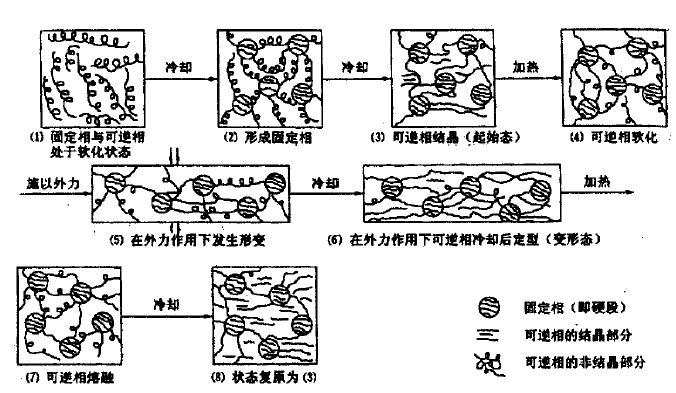
\includegraphics[width=0.75\textwidth]{figures/figure1}
 % \caption[这里的文字将会显示在 listoffigure 中]{这里的文字将会显示在正文中}
 \caption{热塑性形状记忆聚氨酯的形状记忆机理示意图}\label{fig:diagram}
\end{figure}


\subsection{形状记忆聚氨酯的研究进展}
%\label{sec:requirements}
首例SMPU是日本Mitsubishi公司开发成功的……。

\subsection{水系聚氨酯及聚氨酯整理剂}

水系聚氨酯的形态对其流动性,成膜性及加工织物的性能有重要影响,一般分为三种类型\cite{Jiang2005Size} ,如表 \ref{tab:category}所示。

\begin{table}[hbt]
  \centering
  \caption{水系聚氨酯分类} \label{tab:category}
  \begin{tabular*}{0.9\textwidth}{@{\extracolsep{\fill}}cccc}
  \toprule
    类别			&水溶型		&胶体分散型		&乳液型 \\
  \midrule
    状态			&溶解$\sim$胶束	&分散		&白浊 \\
    外观			&水溶型		&胶体分散型		&乳液型 \\
    粒径$/\mu m$	&$<0.001$		&$0.001-0.1$		&$>0.1$ \\
    重均分子量	&$1000\sim 10000$	&数千$\sim 20$万 &$>5000$ \\
  \bottomrule
  \end{tabular*}
\end{table}

\subsubsection{四级节标题}

根据需要,也可设四级节标题。

由于它们对纤维织物的浸透性和亲和性不同,因此在纺织品染整加工中的用途也有差别,其中以水溶型和乳液型产品较为常用。另外,水系聚氨酯又有反应性和非反应性之分。虽然它们的共同特点是分子结构中不含异氰酸酯基,但前者是用封闭剂将异氰酸酯基暂时封闭,在纺织品整理时复出。相互交联反应形成三维网状结构而固着在织物表面。
……


\section{常见问题和疑难解答}

如果您遇到\href{https://bithesis.bitnp.net/faq/char-missing.html}{生僻字无法显示}、
\href{https://bithesis.bitnp.net/faq/enumitem-nosep.html}{列表项间距过大}、
\href{https://bithesis.bitnp.net/faq/longtable.html}{三线表需要跨页}等问题,
请参考\textcolor{magenta}{\href{https://bithesis.bitnp.net/faq/}{在线文档的「疑难杂症」部分}}。
